% SOURCE: editor_ordering_bootstrap_20260726.json fields results.*.contrasts.*.{observed_diff,ci95,p_two_sided}.
% !TEX encoding = UTF-8 Unicode
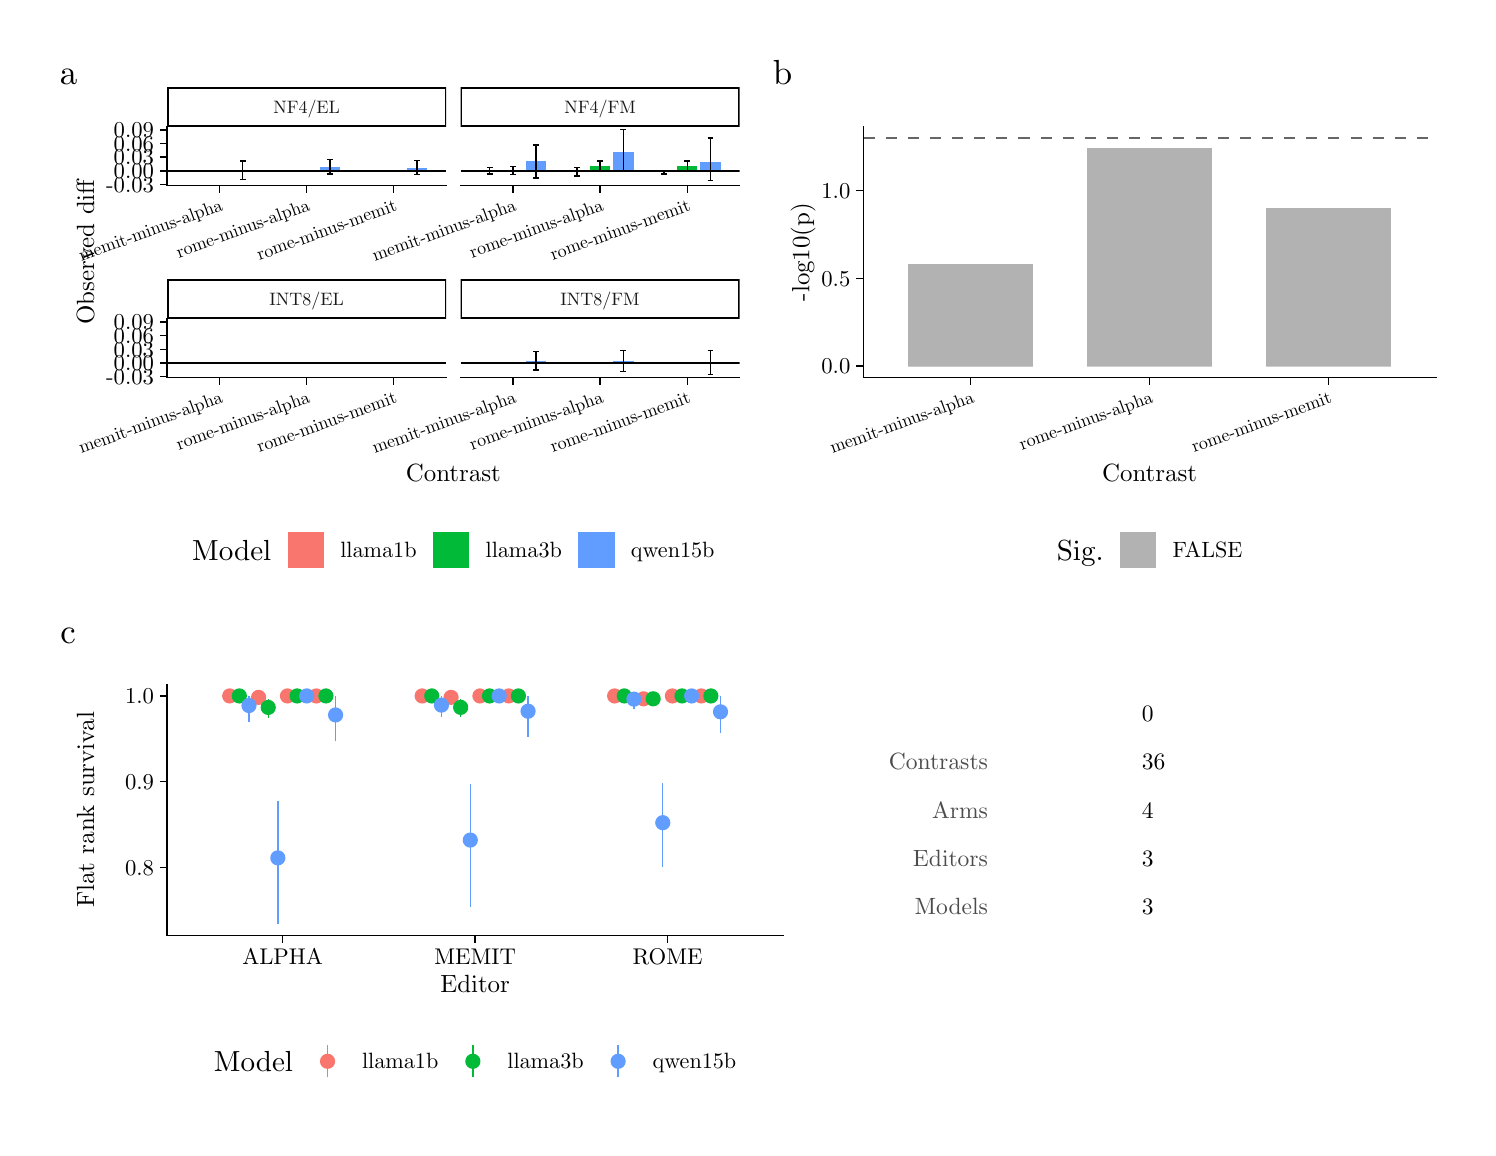
\begin{tikzpicture}[x=1pt,y=1pt]
\definecolor{fillColor}{RGB}{255,255,255}
\path[use as bounding box,fill=fillColor,fill opacity=0.00] (0,0) rectangle (520.34,397.48);
\begin{scope}
\path[clip] (  0.00,  0.00) rectangle (520.34,397.48);
\definecolor{drawColor}{RGB}{255,255,255}
\definecolor{fillColor}{RGB}{255,255,255}

\path[draw=drawColor,line width= 0.6pt,line join=round,line cap=round,fill=fillColor] (  0.00,  0.00) rectangle (520.34,397.48);
\end{scope}
\begin{scope}
\path[clip] (  5.50,190.23) rectangle (263.24,391.98);
\definecolor{drawColor}{RGB}{255,255,255}
\definecolor{fillColor}{RGB}{255,255,255}

\path[draw=drawColor,line width= 0.5pt,line join=round,line cap=round,fill=fillColor] (  5.50,190.23) rectangle (263.24,391.98);
\end{scope}
\begin{scope}
\path[clip] (263.24,190.23) rectangle (514.84,391.98);
\definecolor{drawColor}{RGB}{255,255,255}
\definecolor{fillColor}{RGB}{255,255,255}

\path[draw=drawColor,line width= 0.5pt,line join=round,line cap=round,fill=fillColor] (263.24,190.23) rectangle (514.84,391.98);
\end{scope}
\begin{scope}
\path[clip] ( 50.40,340.52) rectangle (151.20,361.72);
\definecolor{fillColor}{RGB}{255,255,255}

\path[fill=fillColor] ( 50.40,340.52) rectangle (151.20,361.72);
\definecolor{fillColor}{RGB}{248,118,109}

\path[fill=fillColor] (120.22,345.75) rectangle (127.57,345.75);

\path[fill=fillColor] ( 88.73,345.75) rectangle ( 96.07,345.75);

\path[fill=fillColor] ( 57.23,345.75) rectangle ( 64.58,345.75);
\definecolor{fillColor}{RGB}{0,186,56}

\path[fill=fillColor] (128.62,345.75) rectangle (135.97,345.75);

\path[fill=fillColor] ( 97.12,345.75) rectangle (104.47,345.75);

\path[fill=fillColor] ( 65.63,345.75) rectangle ( 72.98,345.75);
\definecolor{fillColor}{RGB}{97,156,255}

\path[fill=fillColor] (137.02,345.75) rectangle (144.37,346.89);

\path[fill=fillColor] (105.52,345.75) rectangle (112.87,346.97);

\path[fill=fillColor] ( 74.03,345.75) rectangle ( 81.38,345.82);
\definecolor{drawColor}{RGB}{0,0,0}

\path[draw=drawColor,line width= 0.5pt,line join=round] (122.85,345.75) --
	(124.95,345.75);

\path[draw=drawColor,line width= 0.5pt,line join=round] (123.90,345.75) --
	(123.90,345.75);

\path[draw=drawColor,line width= 0.5pt,line join=round] (122.85,345.75) --
	(124.95,345.75);

\path[draw=drawColor,line width= 0.5pt,line join=round] ( 91.35,345.75) --
	( 93.45,345.75);

\path[draw=drawColor,line width= 0.5pt,line join=round] ( 92.40,345.75) --
	( 92.40,345.75);

\path[draw=drawColor,line width= 0.5pt,line join=round] ( 91.35,345.75) --
	( 93.45,345.75);

\path[draw=drawColor,line width= 0.5pt,line join=round] ( 59.85,345.75) --
	( 61.95,345.75);

\path[draw=drawColor,line width= 0.5pt,line join=round] ( 60.90,345.75) --
	( 60.90,345.75);

\path[draw=drawColor,line width= 0.5pt,line join=round] ( 59.85,345.75) --
	( 61.95,345.75);

\path[draw=drawColor,line width= 0.5pt,line join=round] (131.25,345.75) --
	(133.35,345.75);

\path[draw=drawColor,line width= 0.5pt,line join=round] (132.30,345.75) --
	(132.30,345.75);

\path[draw=drawColor,line width= 0.5pt,line join=round] (131.25,345.75) --
	(133.35,345.75);

\path[draw=drawColor,line width= 0.5pt,line join=round] ( 99.75,345.75) --
	(101.85,345.75);

\path[draw=drawColor,line width= 0.5pt,line join=round] (100.80,345.75) --
	(100.80,345.75);

\path[draw=drawColor,line width= 0.5pt,line join=round] ( 99.75,345.75) --
	(101.85,345.75);

\path[draw=drawColor,line width= 0.5pt,line join=round] ( 68.25,345.75) --
	( 70.35,345.75);

\path[draw=drawColor,line width= 0.5pt,line join=round] ( 69.30,345.75) --
	( 69.30,345.75);

\path[draw=drawColor,line width= 0.5pt,line join=round] ( 68.25,345.75) --
	( 70.35,345.75);

\path[draw=drawColor,line width= 0.5pt,line join=round] (139.65,349.37) --
	(141.75,349.37);

\path[draw=drawColor,line width= 0.5pt,line join=round] (140.70,349.37) --
	(140.70,344.44);

\path[draw=drawColor,line width= 0.5pt,line join=round] (139.65,344.44) --
	(141.75,344.44);

\path[draw=drawColor,line width= 0.5pt,line join=round] (108.15,349.88) --
	(110.25,349.88);

\path[draw=drawColor,line width= 0.5pt,line join=round] (109.20,349.88) --
	(109.20,344.62);

\path[draw=drawColor,line width= 0.5pt,line join=round] (108.15,344.62) --
	(110.25,344.62);

\path[draw=drawColor,line width= 0.5pt,line join=round] ( 76.65,349.34) --
	( 78.75,349.34);

\path[draw=drawColor,line width= 0.5pt,line join=round] ( 77.70,349.34) --
	( 77.70,342.69);

\path[draw=drawColor,line width= 0.5pt,line join=round] ( 76.65,342.69) --
	( 78.75,342.69);

\path[draw=drawColor,line width= 0.5pt,line join=round] ( 50.40,345.75) -- (151.20,345.75);
\end{scope}
\begin{scope}
\path[clip] ( 50.40,271.09) rectangle (151.20,292.29);
\definecolor{fillColor}{RGB}{255,255,255}

\path[fill=fillColor] ( 50.40,271.09) rectangle (151.20,292.29);
\definecolor{fillColor}{RGB}{248,118,109}

\path[fill=fillColor] (120.22,276.32) rectangle (127.57,276.32);

\path[fill=fillColor] ( 88.73,276.32) rectangle ( 96.07,276.32);

\path[fill=fillColor] ( 57.23,276.32) rectangle ( 64.58,276.32);
\definecolor{fillColor}{RGB}{0,186,56}

\path[fill=fillColor] (128.62,276.32) rectangle (135.97,276.32);

\path[fill=fillColor] ( 97.12,276.32) rectangle (104.47,276.32);

\path[fill=fillColor] ( 65.63,276.32) rectangle ( 72.98,276.32);
\definecolor{fillColor}{RGB}{97,156,255}

\path[fill=fillColor] (137.02,276.32) rectangle (144.37,276.32);

\path[fill=fillColor] (105.52,276.32) rectangle (112.87,276.32);

\path[fill=fillColor] ( 74.03,276.32) rectangle ( 81.38,276.32);
\definecolor{drawColor}{RGB}{0,0,0}

\path[draw=drawColor,line width= 0.5pt,line join=round] (122.85,276.32) --
	(124.95,276.32);

\path[draw=drawColor,line width= 0.5pt,line join=round] (123.90,276.32) --
	(123.90,276.32);

\path[draw=drawColor,line width= 0.5pt,line join=round] (122.85,276.32) --
	(124.95,276.32);

\path[draw=drawColor,line width= 0.5pt,line join=round] ( 91.35,276.32) --
	( 93.45,276.32);

\path[draw=drawColor,line width= 0.5pt,line join=round] ( 92.40,276.32) --
	( 92.40,276.32);

\path[draw=drawColor,line width= 0.5pt,line join=round] ( 91.35,276.32) --
	( 93.45,276.32);

\path[draw=drawColor,line width= 0.5pt,line join=round] ( 59.85,276.32) --
	( 61.95,276.32);

\path[draw=drawColor,line width= 0.5pt,line join=round] ( 60.90,276.32) --
	( 60.90,276.32);

\path[draw=drawColor,line width= 0.5pt,line join=round] ( 59.85,276.32) --
	( 61.95,276.32);

\path[draw=drawColor,line width= 0.5pt,line join=round] (131.25,276.32) --
	(133.35,276.32);

\path[draw=drawColor,line width= 0.5pt,line join=round] (132.30,276.32) --
	(132.30,276.32);

\path[draw=drawColor,line width= 0.5pt,line join=round] (131.25,276.32) --
	(133.35,276.32);

\path[draw=drawColor,line width= 0.5pt,line join=round] ( 99.75,276.32) --
	(101.85,276.32);

\path[draw=drawColor,line width= 0.5pt,line join=round] (100.80,276.32) --
	(100.80,276.32);

\path[draw=drawColor,line width= 0.5pt,line join=round] ( 99.75,276.32) --
	(101.85,276.32);

\path[draw=drawColor,line width= 0.5pt,line join=round] ( 68.25,276.32) --
	( 70.35,276.32);

\path[draw=drawColor,line width= 0.5pt,line join=round] ( 69.30,276.32) --
	( 69.30,276.32);

\path[draw=drawColor,line width= 0.5pt,line join=round] ( 68.25,276.32) --
	( 70.35,276.32);

\path[draw=drawColor,line width= 0.5pt,line join=round] (139.65,276.32) --
	(141.75,276.32);

\path[draw=drawColor,line width= 0.5pt,line join=round] (140.70,276.32) --
	(140.70,276.32);

\path[draw=drawColor,line width= 0.5pt,line join=round] (139.65,276.32) --
	(141.75,276.32);

\path[draw=drawColor,line width= 0.5pt,line join=round] (108.15,276.32) --
	(110.25,276.32);

\path[draw=drawColor,line width= 0.5pt,line join=round] (109.20,276.32) --
	(109.20,276.32);

\path[draw=drawColor,line width= 0.5pt,line join=round] (108.15,276.32) --
	(110.25,276.32);

\path[draw=drawColor,line width= 0.5pt,line join=round] ( 76.65,276.32) --
	( 78.75,276.32);

\path[draw=drawColor,line width= 0.5pt,line join=round] ( 77.70,276.32) --
	( 77.70,276.32);

\path[draw=drawColor,line width= 0.5pt,line join=round] ( 76.65,276.32) --
	( 78.75,276.32);

\path[draw=drawColor,line width= 0.5pt,line join=round] ( 50.40,276.32) -- (151.20,276.32);
\end{scope}
\begin{scope}
\path[clip] (156.45,340.52) rectangle (257.24,361.72);
\definecolor{fillColor}{RGB}{255,255,255}

\path[fill=fillColor] (156.45,340.52) rectangle (257.24,361.72);
\definecolor{fillColor}{RGB}{248,118,109}

\path[fill=fillColor] (226.27,345.47) rectangle (233.61,345.75);

\path[fill=fillColor] (194.77,345.47) rectangle (202.12,345.75);

\path[fill=fillColor] (163.27,345.75) rectangle (170.62,345.75);
\definecolor{fillColor}{RGB}{0,186,56}

\path[fill=fillColor] (234.66,345.75) rectangle (242.01,347.39);

\path[fill=fillColor] (203.17,345.75) rectangle (210.52,347.40);

\path[fill=fillColor] (171.67,345.75) rectangle (179.02,345.76);
\definecolor{fillColor}{RGB}{97,156,255}

\path[fill=fillColor] (243.06,345.75) rectangle (250.41,349.08);

\path[fill=fillColor] (211.57,345.75) rectangle (218.92,352.49);

\path[fill=fillColor] (180.07,345.75) rectangle (187.42,349.16);
\definecolor{drawColor}{RGB}{0,0,0}

\path[draw=drawColor,line width= 0.5pt,line join=round] (228.89,345.75) --
	(230.99,345.75);

\path[draw=drawColor,line width= 0.5pt,line join=round] (229.94,345.75) --
	(229.94,344.63);

\path[draw=drawColor,line width= 0.5pt,line join=round] (228.89,344.63) --
	(230.99,344.63);

\path[draw=drawColor,line width= 0.5pt,line join=round] (197.39,346.85) --
	(199.49,346.85);

\path[draw=drawColor,line width= 0.5pt,line join=round] (198.44,346.85) --
	(198.44,343.81);

\path[draw=drawColor,line width= 0.5pt,line join=round] (197.39,343.81) --
	(199.49,343.81);

\path[draw=drawColor,line width= 0.5pt,line join=round] (165.89,346.85) --
	(167.99,346.85);

\path[draw=drawColor,line width= 0.5pt,line join=round] (166.94,346.85) --
	(166.94,344.64);

\path[draw=drawColor,line width= 0.5pt,line join=round] (165.89,344.64) --
	(167.99,344.64);

\path[draw=drawColor,line width= 0.5pt,line join=round] (237.29,349.31) --
	(239.39,349.31);

\path[draw=drawColor,line width= 0.5pt,line join=round] (238.34,349.31) --
	(238.34,345.47);

\path[draw=drawColor,line width= 0.5pt,line join=round] (237.29,345.47) --
	(239.39,345.47);

\path[draw=drawColor,line width= 0.5pt,line join=round] (205.79,349.31) --
	(207.89,349.31);

\path[draw=drawColor,line width= 0.5pt,line join=round] (206.84,349.31) --
	(206.84,345.75);

\path[draw=drawColor,line width= 0.5pt,line join=round] (205.79,345.75) --
	(207.89,345.75);

\path[draw=drawColor,line width= 0.5pt,line join=round] (174.29,347.39) --
	(176.39,347.39);

\path[draw=drawColor,line width= 0.5pt,line join=round] (175.34,347.39) --
	(175.34,344.38);

\path[draw=drawColor,line width= 0.5pt,line join=round] (174.29,344.38) --
	(176.39,344.38);

\path[draw=drawColor,line width= 0.5pt,line join=round] (245.69,357.56) --
	(247.79,357.56);

\path[draw=drawColor,line width= 0.5pt,line join=round] (246.74,357.56) --
	(246.74,342.28);

\path[draw=drawColor,line width= 0.5pt,line join=round] (245.69,342.28) --
	(247.79,342.28);

\path[draw=drawColor,line width= 0.5pt,line join=round] (214.19,360.75) --
	(216.29,360.75);

\path[draw=drawColor,line width= 0.5pt,line join=round] (215.24,360.75) --
	(215.24,345.62);

\path[draw=drawColor,line width= 0.5pt,line join=round] (214.19,345.62) --
	(216.29,345.62);

\path[draw=drawColor,line width= 0.5pt,line join=round] (182.69,355.03) --
	(184.79,355.03);

\path[draw=drawColor,line width= 0.5pt,line join=round] (183.74,355.03) --
	(183.74,343.11);

\path[draw=drawColor,line width= 0.5pt,line join=round] (182.69,343.11) --
	(184.79,343.11);

\path[draw=drawColor,line width= 0.5pt,line join=round] (156.45,345.75) -- (257.24,345.75);
\end{scope}
\begin{scope}
\path[clip] (156.45,271.09) rectangle (257.24,292.29);
\definecolor{fillColor}{RGB}{255,255,255}

\path[fill=fillColor] (156.45,271.09) rectangle (257.24,292.29);
\definecolor{fillColor}{RGB}{248,118,109}

\path[fill=fillColor] (226.27,276.32) rectangle (233.61,276.32);

\path[fill=fillColor] (194.77,276.32) rectangle (202.12,276.32);

\path[fill=fillColor] (163.27,276.32) rectangle (170.62,276.32);
\definecolor{fillColor}{RGB}{0,186,56}

\path[fill=fillColor] (234.66,276.32) rectangle (242.01,276.32);

\path[fill=fillColor] (203.17,276.32) rectangle (210.52,276.32);

\path[fill=fillColor] (171.67,276.32) rectangle (179.02,276.32);
\definecolor{fillColor}{RGB}{97,156,255}

\path[fill=fillColor] (243.06,276.20) rectangle (250.41,276.32);

\path[fill=fillColor] (211.57,276.32) rectangle (218.92,276.91);

\path[fill=fillColor] (180.07,276.32) rectangle (187.42,277.03);
\definecolor{drawColor}{RGB}{0,0,0}

\path[draw=drawColor,line width= 0.5pt,line join=round] (228.89,276.32) --
	(230.99,276.32);

\path[draw=drawColor,line width= 0.5pt,line join=round] (229.94,276.32) --
	(229.94,276.32);

\path[draw=drawColor,line width= 0.5pt,line join=round] (228.89,276.32) --
	(230.99,276.32);

\path[draw=drawColor,line width= 0.5pt,line join=round] (197.39,276.32) --
	(199.49,276.32);

\path[draw=drawColor,line width= 0.5pt,line join=round] (198.44,276.32) --
	(198.44,276.32);

\path[draw=drawColor,line width= 0.5pt,line join=round] (197.39,276.32) --
	(199.49,276.32);

\path[draw=drawColor,line width= 0.5pt,line join=round] (165.89,276.32) --
	(167.99,276.32);

\path[draw=drawColor,line width= 0.5pt,line join=round] (166.94,276.32) --
	(166.94,276.32);

\path[draw=drawColor,line width= 0.5pt,line join=round] (165.89,276.32) --
	(167.99,276.32);

\path[draw=drawColor,line width= 0.5pt,line join=round] (237.29,276.32) --
	(239.39,276.32);

\path[draw=drawColor,line width= 0.5pt,line join=round] (238.34,276.32) --
	(238.34,276.32);

\path[draw=drawColor,line width= 0.5pt,line join=round] (237.29,276.32) --
	(239.39,276.32);

\path[draw=drawColor,line width= 0.5pt,line join=round] (205.79,276.32) --
	(207.89,276.32);

\path[draw=drawColor,line width= 0.5pt,line join=round] (206.84,276.32) --
	(206.84,276.32);

\path[draw=drawColor,line width= 0.5pt,line join=round] (205.79,276.32) --
	(207.89,276.32);

\path[draw=drawColor,line width= 0.5pt,line join=round] (174.29,276.32) --
	(176.39,276.32);

\path[draw=drawColor,line width= 0.5pt,line join=round] (175.34,276.32) --
	(175.34,276.32);

\path[draw=drawColor,line width= 0.5pt,line join=round] (174.29,276.32) --
	(176.39,276.32);

\path[draw=drawColor,line width= 0.5pt,line join=round] (245.69,280.79) --
	(247.79,280.79);

\path[draw=drawColor,line width= 0.5pt,line join=round] (246.74,280.79) --
	(246.74,272.05);

\path[draw=drawColor,line width= 0.5pt,line join=round] (245.69,272.05) --
	(247.79,272.05);

\path[draw=drawColor,line width= 0.5pt,line join=round] (214.19,280.75) --
	(216.29,280.75);

\path[draw=drawColor,line width= 0.5pt,line join=round] (215.24,280.75) --
	(215.24,273.25);

\path[draw=drawColor,line width= 0.5pt,line join=round] (214.19,273.25) --
	(216.29,273.25);

\path[draw=drawColor,line width= 0.5pt,line join=round] (182.69,280.57) --
	(184.79,280.57);

\path[draw=drawColor,line width= 0.5pt,line join=round] (183.74,280.57) --
	(183.74,273.82);

\path[draw=drawColor,line width= 0.5pt,line join=round] (182.69,273.82) --
	(184.79,273.82);

\path[draw=drawColor,line width= 0.5pt,line join=round] (156.45,276.32) -- (257.24,276.32);
\end{scope}
\begin{scope}
\path[clip] ( 50.40,292.29) rectangle (151.20,306.43);
\definecolor{drawColor}{RGB}{0,0,0}
\definecolor{fillColor}{RGB}{255,255,255}

\path[draw=drawColor,line width= 1.1pt,line join=round,line cap=round,fill=fillColor] ( 50.40,292.29) rectangle (151.20,306.43);
\definecolor{drawColor}{gray}{0.10}

\node[text=drawColor,anchor=base,inner sep=0pt, outer sep=0pt, scale=  0.65] at (100.80,297.12) {INT8/EL};
\end{scope}
\begin{scope}
\path[clip] (156.45,292.29) rectangle (257.24,306.43);
\definecolor{drawColor}{RGB}{0,0,0}
\definecolor{fillColor}{RGB}{255,255,255}

\path[draw=drawColor,line width= 1.1pt,line join=round,line cap=round,fill=fillColor] (156.45,292.29) rectangle (257.24,306.43);
\definecolor{drawColor}{gray}{0.10}

\node[text=drawColor,anchor=base,inner sep=0pt, outer sep=0pt, scale=  0.65] at (206.84,297.12) {INT8/FM};
\end{scope}
\begin{scope}
\path[clip] (  0.00,  0.00) rectangle (520.34,397.48);
\definecolor{drawColor}{RGB}{0,0,0}

\path[draw=drawColor,line width= 0.5pt,line join=round,line cap=rect] ( 50.40,340.52) --
	(151.20,340.52);
\end{scope}
\begin{scope}
\path[clip] (  0.00,  0.00) rectangle (520.34,397.48);
\definecolor{drawColor}{RGB}{0,0,0}

\path[draw=drawColor,line width= 0.5pt,line join=round] ( 69.30,337.89) --
	( 69.30,340.52);

\path[draw=drawColor,line width= 0.5pt,line join=round] (100.80,337.89) --
	(100.80,340.52);

\path[draw=drawColor,line width= 0.5pt,line join=round] (132.30,337.89) --
	(132.30,340.52);
\end{scope}
\begin{scope}
\path[clip] (  0.00,  0.00) rectangle (520.34,397.48);
\definecolor{drawColor}{RGB}{0,0,0}

\node[text=drawColor,rotate= 20.00,anchor=base east,inner sep=0pt, outer sep=0pt, scale=  0.65] at ( 70.83,331.59) {memit-minus-alpha};

\node[text=drawColor,rotate= 20.00,anchor=base east,inner sep=0pt, outer sep=0pt, scale=  0.65] at (102.33,331.59) {rome-minus-alpha};

\node[text=drawColor,rotate= 20.00,anchor=base east,inner sep=0pt, outer sep=0pt, scale=  0.65] at (133.83,331.59) {rome-minus-memit};
\end{scope}
\begin{scope}
\path[clip] (  0.00,  0.00) rectangle (520.34,397.48);
\definecolor{drawColor}{RGB}{0,0,0}

\path[draw=drawColor,line width= 0.5pt,line join=round,line cap=rect] (156.45,340.52) --
	(257.24,340.52);
\end{scope}
\begin{scope}
\path[clip] (  0.00,  0.00) rectangle (520.34,397.48);
\definecolor{drawColor}{RGB}{0,0,0}

\path[draw=drawColor,line width= 0.5pt,line join=round] (175.34,337.89) --
	(175.34,340.52);

\path[draw=drawColor,line width= 0.5pt,line join=round] (206.84,337.89) --
	(206.84,340.52);

\path[draw=drawColor,line width= 0.5pt,line join=round] (238.34,337.89) --
	(238.34,340.52);
\end{scope}
\begin{scope}
\path[clip] (  0.00,  0.00) rectangle (520.34,397.48);
\definecolor{drawColor}{RGB}{0,0,0}

\node[text=drawColor,rotate= 20.00,anchor=base east,inner sep=0pt, outer sep=0pt, scale=  0.65] at (176.88,331.59) {memit-minus-alpha};

\node[text=drawColor,rotate= 20.00,anchor=base east,inner sep=0pt, outer sep=0pt, scale=  0.65] at (208.37,331.59) {rome-minus-alpha};

\node[text=drawColor,rotate= 20.00,anchor=base east,inner sep=0pt, outer sep=0pt, scale=  0.65] at (239.87,331.59) {rome-minus-memit};
\end{scope}
\begin{scope}
\path[clip] ( 50.40,361.72) rectangle (151.20,375.86);
\definecolor{drawColor}{RGB}{0,0,0}
\definecolor{fillColor}{RGB}{255,255,255}

\path[draw=drawColor,line width= 1.1pt,line join=round,line cap=round,fill=fillColor] ( 50.40,361.72) rectangle (151.20,375.86);
\definecolor{drawColor}{gray}{0.10}

\node[text=drawColor,anchor=base,inner sep=0pt, outer sep=0pt, scale=  0.65] at (100.80,366.55) {NF4/EL};
\end{scope}
\begin{scope}
\path[clip] (156.45,361.72) rectangle (257.24,375.86);
\definecolor{drawColor}{RGB}{0,0,0}
\definecolor{fillColor}{RGB}{255,255,255}

\path[draw=drawColor,line width= 1.1pt,line join=round,line cap=round,fill=fillColor] (156.45,361.72) rectangle (257.24,375.86);
\definecolor{drawColor}{gray}{0.10}

\node[text=drawColor,anchor=base,inner sep=0pt, outer sep=0pt, scale=  0.65] at (206.84,366.55) {NF4/FM};
\end{scope}
\begin{scope}
\path[clip] (  0.00,  0.00) rectangle (520.34,397.48);
\definecolor{drawColor}{RGB}{0,0,0}

\path[draw=drawColor,line width= 0.5pt,line join=round,line cap=rect] ( 50.40,271.09) --
	(151.20,271.09);
\end{scope}
\begin{scope}
\path[clip] (  0.00,  0.00) rectangle (520.34,397.48);
\definecolor{drawColor}{RGB}{0,0,0}

\path[draw=drawColor,line width= 0.5pt,line join=round] ( 69.30,268.47) --
	( 69.30,271.09);

\path[draw=drawColor,line width= 0.5pt,line join=round] (100.80,268.47) --
	(100.80,271.09);

\path[draw=drawColor,line width= 0.5pt,line join=round] (132.30,268.47) --
	(132.30,271.09);
\end{scope}
\begin{scope}
\path[clip] (  0.00,  0.00) rectangle (520.34,397.48);
\definecolor{drawColor}{RGB}{0,0,0}

\node[text=drawColor,rotate= 20.00,anchor=base east,inner sep=0pt, outer sep=0pt, scale=  0.65] at ( 70.83,262.16) {memit-minus-alpha};

\node[text=drawColor,rotate= 20.00,anchor=base east,inner sep=0pt, outer sep=0pt, scale=  0.65] at (102.33,262.16) {rome-minus-alpha};

\node[text=drawColor,rotate= 20.00,anchor=base east,inner sep=0pt, outer sep=0pt, scale=  0.65] at (133.83,262.16) {rome-minus-memit};
\end{scope}
\begin{scope}
\path[clip] (  0.00,  0.00) rectangle (520.34,397.48);
\definecolor{drawColor}{RGB}{0,0,0}

\path[draw=drawColor,line width= 0.5pt,line join=round,line cap=rect] (156.45,271.09) --
	(257.24,271.09);
\end{scope}
\begin{scope}
\path[clip] (  0.00,  0.00) rectangle (520.34,397.48);
\definecolor{drawColor}{RGB}{0,0,0}

\path[draw=drawColor,line width= 0.5pt,line join=round] (175.34,268.47) --
	(175.34,271.09);

\path[draw=drawColor,line width= 0.5pt,line join=round] (206.84,268.47) --
	(206.84,271.09);

\path[draw=drawColor,line width= 0.5pt,line join=round] (238.34,268.47) --
	(238.34,271.09);
\end{scope}
\begin{scope}
\path[clip] (  0.00,  0.00) rectangle (520.34,397.48);
\definecolor{drawColor}{RGB}{0,0,0}

\node[text=drawColor,rotate= 20.00,anchor=base east,inner sep=0pt, outer sep=0pt, scale=  0.65] at (176.88,262.16) {memit-minus-alpha};

\node[text=drawColor,rotate= 20.00,anchor=base east,inner sep=0pt, outer sep=0pt, scale=  0.65] at (208.37,262.16) {rome-minus-alpha};

\node[text=drawColor,rotate= 20.00,anchor=base east,inner sep=0pt, outer sep=0pt, scale=  0.65] at (239.87,262.16) {rome-minus-memit};
\end{scope}
\begin{scope}
\path[clip] (  0.00,  0.00) rectangle (520.34,397.48);
\definecolor{drawColor}{RGB}{0,0,0}

\path[draw=drawColor,line width= 0.5pt,line join=round,line cap=rect] ( 50.40,340.52) --
	( 50.40,361.72);
\end{scope}
\begin{scope}
\path[clip] (  0.00,  0.00) rectangle (520.34,397.48);
\definecolor{drawColor}{RGB}{0,0,0}

\node[text=drawColor,anchor=base east,inner sep=0pt, outer sep=0pt, scale=  0.82] at ( 45.68,337.99) {-0.03};

\node[text=drawColor,anchor=base east,inner sep=0pt, outer sep=0pt, scale=  0.82] at ( 45.68,342.92) {0.00};

\node[text=drawColor,anchor=base east,inner sep=0pt, outer sep=0pt, scale=  0.82] at ( 45.68,347.86) {0.03};

\node[text=drawColor,anchor=base east,inner sep=0pt, outer sep=0pt, scale=  0.82] at ( 45.68,352.79) {0.06};

\node[text=drawColor,anchor=base east,inner sep=0pt, outer sep=0pt, scale=  0.82] at ( 45.68,357.72) {0.09};
\end{scope}
\begin{scope}
\path[clip] (  0.00,  0.00) rectangle (520.34,397.48);
\definecolor{drawColor}{RGB}{0,0,0}

\path[draw=drawColor,line width= 0.5pt,line join=round] ( 47.78,340.81) --
	( 50.40,340.81);

\path[draw=drawColor,line width= 0.5pt,line join=round] ( 47.78,345.75) --
	( 50.40,345.75);

\path[draw=drawColor,line width= 0.5pt,line join=round] ( 47.78,350.68) --
	( 50.40,350.68);

\path[draw=drawColor,line width= 0.5pt,line join=round] ( 47.78,355.61) --
	( 50.40,355.61);

\path[draw=drawColor,line width= 0.5pt,line join=round] ( 47.78,360.55) --
	( 50.40,360.55);
\end{scope}
\begin{scope}
\path[clip] (  0.00,  0.00) rectangle (520.34,397.48);
\definecolor{drawColor}{RGB}{0,0,0}

\path[draw=drawColor,line width= 0.5pt,line join=round,line cap=rect] ( 50.40,271.09) --
	( 50.40,292.29);
\end{scope}
\begin{scope}
\path[clip] (  0.00,  0.00) rectangle (520.34,397.48);
\definecolor{drawColor}{RGB}{0,0,0}

\node[text=drawColor,anchor=base east,inner sep=0pt, outer sep=0pt, scale=  0.82] at ( 45.68,268.56) {-0.03};

\node[text=drawColor,anchor=base east,inner sep=0pt, outer sep=0pt, scale=  0.82] at ( 45.68,273.49) {0.00};

\node[text=drawColor,anchor=base east,inner sep=0pt, outer sep=0pt, scale=  0.82] at ( 45.68,278.43) {0.03};

\node[text=drawColor,anchor=base east,inner sep=0pt, outer sep=0pt, scale=  0.82] at ( 45.68,283.36) {0.06};

\node[text=drawColor,anchor=base east,inner sep=0pt, outer sep=0pt, scale=  0.82] at ( 45.68,288.29) {0.09};
\end{scope}
\begin{scope}
\path[clip] (  0.00,  0.00) rectangle (520.34,397.48);
\definecolor{drawColor}{RGB}{0,0,0}

\path[draw=drawColor,line width= 0.5pt,line join=round] ( 47.78,271.38) --
	( 50.40,271.38);

\path[draw=drawColor,line width= 0.5pt,line join=round] ( 47.78,276.32) --
	( 50.40,276.32);

\path[draw=drawColor,line width= 0.5pt,line join=round] ( 47.78,281.25) --
	( 50.40,281.25);

\path[draw=drawColor,line width= 0.5pt,line join=round] ( 47.78,286.19) --
	( 50.40,286.19);

\path[draw=drawColor,line width= 0.5pt,line join=round] ( 47.78,291.12) --
	( 50.40,291.12);
\end{scope}
\begin{scope}
\path[clip] (  0.00,  0.00) rectangle (520.34,397.48);
\definecolor{drawColor}{RGB}{0,0,0}

\node[text=drawColor,anchor=base,inner sep=0pt, outer sep=0pt, scale=  0.90] at (153.82,233.43) {Contrast};
\end{scope}
\begin{scope}
\path[clip] (  0.00,  0.00) rectangle (520.34,397.48);
\definecolor{drawColor}{RGB}{0,0,0}

\node[text=drawColor,rotate= 90.00,anchor=base,inner sep=0pt, outer sep=0pt, scale=  0.90] at ( 24.00,316.40) {Observed diff};
\end{scope}
\begin{scope}
\path[clip] (  0.00,  0.00) rectangle (520.34,397.48);
\definecolor{fillColor}{RGB}{255,255,255}

\path[fill=fillColor] ( 54.20,196.23) rectangle (253.45,221.18);
\end{scope}
\begin{scope}
\path[clip] (  0.00,  0.00) rectangle (520.34,397.48);
\definecolor{drawColor}{RGB}{0,0,0}

\node[text=drawColor,anchor=base west,inner sep=0pt, outer sep=0pt, scale=  1.05] at ( 59.45,205.09) {Model};
\end{scope}
\begin{scope}
\path[clip] (  0.00,  0.00) rectangle (520.34,397.48);
\definecolor{fillColor}{RGB}{255,255,255}

\path[fill=fillColor] ( 93.27,201.48) rectangle (107.73,215.93);
\definecolor{fillColor}{RGB}{248,118,109}

\path[fill=fillColor] ( 93.95,202.15) rectangle (107.05,215.25);
\end{scope}
\begin{scope}
\path[clip] (  0.00,  0.00) rectangle (520.34,397.48);
\definecolor{fillColor}{RGB}{255,255,255}

\path[fill=fillColor] (145.77,201.48) rectangle (160.23,215.93);
\definecolor{fillColor}{RGB}{0,186,56}

\path[fill=fillColor] (146.45,202.15) rectangle (159.55,215.25);
\end{scope}
\begin{scope}
\path[clip] (  0.00,  0.00) rectangle (520.34,397.48);
\definecolor{fillColor}{RGB}{255,255,255}

\path[fill=fillColor] (198.28,201.48) rectangle (212.73,215.93);
\definecolor{fillColor}{RGB}{97,156,255}

\path[fill=fillColor] (198.96,202.15) rectangle (212.05,215.25);
\end{scope}
\begin{scope}
\path[clip] (  0.00,  0.00) rectangle (520.34,397.48);
\definecolor{drawColor}{RGB}{0,0,0}

\node[text=drawColor,anchor=base west,inner sep=0pt, outer sep=0pt, scale=  0.80] at (112.98,205.95) {llama1b};
\end{scope}
\begin{scope}
\path[clip] (  0.00,  0.00) rectangle (520.34,397.48);
\definecolor{drawColor}{RGB}{0,0,0}

\node[text=drawColor,anchor=base west,inner sep=0pt, outer sep=0pt, scale=  0.80] at (165.48,205.95) {llama3b};
\end{scope}
\begin{scope}
\path[clip] (  0.00,  0.00) rectangle (520.34,397.48);
\definecolor{drawColor}{RGB}{0,0,0}

\node[text=drawColor,anchor=base west,inner sep=0pt, outer sep=0pt, scale=  0.80] at (217.98,205.95) {qwen15b};
\end{scope}
\begin{scope}
\path[clip] (  0.00,  0.00) rectangle (520.34,397.48);
\definecolor{drawColor}{RGB}{0,0,0}

\node[text=drawColor,anchor=base,inner sep=0pt, outer sep=0pt, scale=  1.26] at ( 14.65,377.08) {a};
\end{scope}
\begin{scope}
\path[clip] (302.01,271.09) rectangle (508.84,361.72);
\definecolor{fillColor}{RGB}{255,255,255}

\path[fill=fillColor] (302.01,271.09) rectangle (508.84,361.72);
\definecolor{fillColor}{gray}{0.70}

\path[fill=fillColor] (447.44,275.21) rectangle (492.69,275.21);

\path[fill=fillColor] (382.80,275.21) rectangle (428.05,275.21);

\path[fill=fillColor] (318.17,275.21) rectangle (363.41,275.21);

\path[fill=fillColor] (447.44,275.21) rectangle (492.69,283.48);

\path[fill=fillColor] (382.80,275.21) rectangle (428.05,279.09);

\path[fill=fillColor] (318.17,275.21) rectangle (363.41,275.21);

\path[fill=fillColor] (447.44,275.21) rectangle (492.69,275.21);

\path[fill=fillColor] (382.80,275.21) rectangle (428.05,275.21);

\path[fill=fillColor] (318.17,275.21) rectangle (363.41,275.21);

\path[fill=fillColor] (447.44,275.21) rectangle (492.69,275.21);

\path[fill=fillColor] (382.80,275.21) rectangle (428.05,275.21);

\path[fill=fillColor] (318.17,275.21) rectangle (363.41,275.21);

\path[fill=fillColor] (447.44,275.21) rectangle (492.69,275.21);

\path[fill=fillColor] (382.80,275.21) rectangle (428.05,275.21);

\path[fill=fillColor] (318.17,275.21) rectangle (363.41,275.21);

\path[fill=fillColor] (447.44,275.21) rectangle (492.69,332.27);

\path[fill=fillColor] (382.80,275.21) rectangle (428.05,353.05);

\path[fill=fillColor] (318.17,275.21) rectangle (363.41,275.70);

\path[fill=fillColor] (447.44,275.21) rectangle (492.69,275.21);

\path[fill=fillColor] (382.80,275.21) rectangle (428.05,275.21);

\path[fill=fillColor] (318.17,275.21) rectangle (363.41,275.21);

\path[fill=fillColor] (447.44,275.21) rectangle (492.69,275.21);

\path[fill=fillColor] (382.80,275.21) rectangle (428.05,275.21);

\path[fill=fillColor] (318.17,275.21) rectangle (363.41,275.21);

\path[fill=fillColor] (447.44,275.21) rectangle (492.69,301.60);

\path[fill=fillColor] (382.80,275.21) rectangle (428.05,300.97);

\path[fill=fillColor] (318.17,275.21) rectangle (363.41,275.91);

\path[fill=fillColor] (447.44,275.21) rectangle (492.69,301.16);

\path[fill=fillColor] (382.80,275.21) rectangle (428.05,353.99);

\path[fill=fillColor] (318.17,275.21) rectangle (363.41,312.07);

\path[fill=fillColor] (447.44,275.21) rectangle (492.69,275.21);

\path[fill=fillColor] (382.80,275.21) rectangle (428.05,275.21);

\path[fill=fillColor] (318.17,275.21) rectangle (363.41,275.21);

\path[fill=fillColor] (447.44,275.21) rectangle (492.69,276.70);

\path[fill=fillColor] (382.80,275.21) rectangle (428.05,281.70);

\path[fill=fillColor] (318.17,275.21) rectangle (363.41,286.36);
\definecolor{drawColor}{gray}{0.40}

\path[draw=drawColor,line width= 0.5pt,dash pattern=on 4pt off 4pt ,line join=round] (302.01,357.60) -- (508.84,357.60);
\end{scope}
\begin{scope}
\path[clip] (  0.00,  0.00) rectangle (520.34,397.48);
\definecolor{drawColor}{RGB}{0,0,0}

\path[draw=drawColor,line width= 0.5pt,line join=round,line cap=rect] (302.01,271.09) --
	(302.01,361.72);
\end{scope}
\begin{scope}
\path[clip] (  0.00,  0.00) rectangle (520.34,397.48);
\definecolor{drawColor}{RGB}{0,0,0}

\node[text=drawColor,anchor=base east,inner sep=0pt, outer sep=0pt, scale=  0.82] at (297.28,272.39) {0.0};

\node[text=drawColor,anchor=base east,inner sep=0pt, outer sep=0pt, scale=  0.82] at (297.28,304.05) {0.5};

\node[text=drawColor,anchor=base east,inner sep=0pt, outer sep=0pt, scale=  0.82] at (297.28,335.71) {1.0};
\end{scope}
\begin{scope}
\path[clip] (  0.00,  0.00) rectangle (520.34,397.48);
\definecolor{drawColor}{RGB}{0,0,0}

\path[draw=drawColor,line width= 0.5pt,line join=round] (299.38,275.21) --
	(302.01,275.21);

\path[draw=drawColor,line width= 0.5pt,line join=round] (299.38,306.87) --
	(302.01,306.87);

\path[draw=drawColor,line width= 0.5pt,line join=round] (299.38,338.54) --
	(302.01,338.54);
\end{scope}
\begin{scope}
\path[clip] (  0.00,  0.00) rectangle (520.34,397.48);
\definecolor{drawColor}{RGB}{0,0,0}

\path[draw=drawColor,line width= 0.5pt,line join=round,line cap=rect] (302.01,271.09) --
	(508.84,271.09);
\end{scope}
\begin{scope}
\path[clip] (  0.00,  0.00) rectangle (520.34,397.48);
\definecolor{drawColor}{RGB}{0,0,0}

\path[draw=drawColor,line width= 0.5pt,line join=round] (340.79,268.47) --
	(340.79,271.09);

\path[draw=drawColor,line width= 0.5pt,line join=round] (405.43,268.47) --
	(405.43,271.09);

\path[draw=drawColor,line width= 0.5pt,line join=round] (470.06,268.47) --
	(470.06,271.09);
\end{scope}
\begin{scope}
\path[clip] (  0.00,  0.00) rectangle (520.34,397.48);
\definecolor{drawColor}{RGB}{0,0,0}

\node[text=drawColor,rotate= 20.00,anchor=base east,inner sep=0pt, outer sep=0pt, scale=  0.65] at (342.32,262.16) {memit-minus-alpha};

\node[text=drawColor,rotate= 20.00,anchor=base east,inner sep=0pt, outer sep=0pt, scale=  0.65] at (406.96,262.16) {rome-minus-alpha};

\node[text=drawColor,rotate= 20.00,anchor=base east,inner sep=0pt, outer sep=0pt, scale=  0.65] at (471.59,262.16) {rome-minus-memit};
\end{scope}
\begin{scope}
\path[clip] (  0.00,  0.00) rectangle (520.34,397.48);
\definecolor{drawColor}{RGB}{0,0,0}

\node[text=drawColor,anchor=base,inner sep=0pt, outer sep=0pt, scale=  0.90] at (405.43,233.43) {Contrast};
\end{scope}
\begin{scope}
\path[clip] (  0.00,  0.00) rectangle (520.34,397.48);
\definecolor{drawColor}{RGB}{0,0,0}

\node[text=drawColor,rotate= 90.00,anchor=base,inner sep=0pt, outer sep=0pt, scale=  0.90] at (282.43,316.40) {-log10(p)};
\end{scope}
\begin{scope}
\path[clip] (  0.00,  0.00) rectangle (520.34,397.48);
\definecolor{fillColor}{RGB}{255,255,255}

\path[fill=fillColor] (366.64,196.23) rectangle (444.22,221.18);
\end{scope}
\begin{scope}
\path[clip] (  0.00,  0.00) rectangle (520.34,397.48);
\definecolor{drawColor}{RGB}{0,0,0}

\node[text=drawColor,anchor=base west,inner sep=0pt, outer sep=0pt, scale=  1.05] at (371.89,205.09) {Sig.};
\end{scope}
\begin{scope}
\path[clip] (  0.00,  0.00) rectangle (520.34,397.48);
\definecolor{fillColor}{RGB}{255,255,255}

\path[fill=fillColor] (394.05,201.48) rectangle (408.50,215.93);
\definecolor{fillColor}{gray}{0.70}

\path[fill=fillColor] (394.73,202.15) rectangle (407.82,215.25);
\end{scope}
\begin{scope}
\path[clip] (  0.00,  0.00) rectangle (520.34,397.48);
\definecolor{drawColor}{RGB}{0,0,0}

\node[text=drawColor,anchor=base west,inner sep=0pt, outer sep=0pt, scale=  0.80] at (413.75,205.95) {FALSE};
\end{scope}
\begin{scope}
\path[clip] (  0.00,  0.00) rectangle (520.34,397.48);
\definecolor{drawColor}{RGB}{0,0,0}

\node[text=drawColor,anchor=base,inner sep=0pt, outer sep=0pt, scale=  1.26] at (272.74,377.08) {b};
\end{scope}
\begin{scope}
\path[clip] (  5.50,  5.50) rectangle (278.96,190.23);
\definecolor{drawColor}{RGB}{255,255,255}
\definecolor{fillColor}{RGB}{255,255,255}

\path[draw=drawColor,line width= 0.5pt,line join=round,line cap=round,fill=fillColor] (  5.50,  5.50) rectangle (278.96,190.23);
\end{scope}
\begin{scope}
\path[clip] (278.96,  5.50) rectangle (514.84,190.23);

\path[] (278.96,  5.50) rectangle (514.84,190.23);
\end{scope}
\begin{scope}
\path[clip] ( 50.40, 69.49) rectangle (272.96,160.12);
\definecolor{fillColor}{RGB}{255,255,255}

\path[fill=fillColor] ( 50.40, 69.49) rectangle (272.96,160.12);
\definecolor{drawColor}{RGB}{248,118,109}

\path[draw=drawColor,line width= 0.5pt,line join=round] (212.10,156.00) -- (212.10,156.00);

\path[draw=drawColor,line width= 0.5pt,line join=round] (142.55,156.00) -- (142.55,156.00);

\path[draw=drawColor,line width= 0.5pt,line join=round] ( 73.01,156.00) -- ( 73.01,156.00);

\path[draw=drawColor,line width= 0.5pt,line join=round] (222.54,152.34) -- (222.54,156.00);

\path[draw=drawColor,line width= 0.5pt,line join=round] (152.99,153.91) -- (152.99,156.00);

\path[draw=drawColor,line width= 0.5pt,line join=round] ( 83.44,153.92) -- ( 83.44,156.00);

\path[draw=drawColor,line width= 0.5pt,line join=round] (232.97,156.00) -- (232.97,156.00);

\path[draw=drawColor,line width= 0.5pt,line join=round] (163.42,156.00) -- (163.42,156.00);

\path[draw=drawColor,line width= 0.5pt,line join=round] ( 93.87,156.00) -- ( 93.87,156.00);

\path[draw=drawColor,line width= 0.5pt,line join=round] (243.40,156.00) -- (243.40,156.00);

\path[draw=drawColor,line width= 0.5pt,line join=round] (173.85,156.00) -- (173.85,156.00);

\path[draw=drawColor,line width= 0.5pt,line join=round] (104.30,156.00) -- (104.30,156.00);
\definecolor{drawColor}{RGB}{0,186,56}

\path[draw=drawColor,line width= 0.5pt,line join=round] (215.58,156.00) -- (215.58,156.00);

\path[draw=drawColor,line width= 0.5pt,line join=round] (146.03,156.00) -- (146.03,156.00);

\path[draw=drawColor,line width= 0.5pt,line join=round] ( 76.48,156.00) -- ( 76.48,156.00);

\path[draw=drawColor,line width= 0.5pt,line join=round] (226.01,152.90) -- (226.01,156.00);

\path[draw=drawColor,line width= 0.5pt,line join=round] (156.46,148.25) -- (156.46,154.97);

\path[draw=drawColor,line width= 0.5pt,line join=round] ( 86.92,148.17) -- ( 86.92,154.96);

\path[draw=drawColor,line width= 0.5pt,line join=round] (236.45,156.00) -- (236.45,156.00);

\path[draw=drawColor,line width= 0.5pt,line join=round] (166.90,156.00) -- (166.90,156.00);

\path[draw=drawColor,line width= 0.5pt,line join=round] ( 97.35,156.00) -- ( 97.35,156.00);

\path[draw=drawColor,line width= 0.5pt,line join=round] (246.88,156.00) -- (246.88,156.00);

\path[draw=drawColor,line width= 0.5pt,line join=round] (177.33,156.00) -- (177.33,156.00);

\path[draw=drawColor,line width= 0.5pt,line join=round] (107.78,156.00) -- (107.78,156.00);
\definecolor{drawColor}{RGB}{97,156,255}

\path[draw=drawColor,line width= 0.5pt,line join=round] (219.06,151.21) -- (219.06,156.00);

\path[draw=drawColor,line width= 0.5pt,line join=round] (149.51,148.48) -- (149.51,156.00);

\path[draw=drawColor,line width= 0.5pt,line join=round] ( 79.96,146.71) -- ( 79.96,156.00);

\path[draw=drawColor,line width= 0.5pt,line join=round] (229.49, 94.32) -- (229.49,124.66);

\path[draw=drawColor,line width= 0.5pt,line join=round] (159.94, 79.62) -- (159.94,124.25);

\path[draw=drawColor,line width= 0.5pt,line join=round] ( 90.39, 73.61) -- ( 90.39,117.97);

\path[draw=drawColor,line width= 0.5pt,line join=round] (239.92,156.00) -- (239.92,156.00);

\path[draw=drawColor,line width= 0.5pt,line join=round] (170.37,156.00) -- (170.37,156.00);

\path[draw=drawColor,line width= 0.5pt,line join=round] (100.83,156.00) -- (100.83,156.00);

\path[draw=drawColor,line width= 0.5pt,line join=round] (250.35,142.60) -- (250.35,156.00);

\path[draw=drawColor,line width= 0.5pt,line join=round] (180.81,141.32) -- (180.81,156.00);

\path[draw=drawColor,line width= 0.5pt,line join=round] (111.26,139.60) -- (111.26,156.00);
\definecolor{drawColor}{RGB}{248,118,109}
\definecolor{fillColor}{RGB}{248,118,109}

\path[draw=drawColor,line width= 0.7pt,line join=round,line cap=round,fill=fillColor] (212.10,156.00) circle (  2.39);

\path[draw=drawColor,line width= 0.7pt,line join=round,line cap=round,fill=fillColor] (142.55,156.00) circle (  2.39);

\path[draw=drawColor,line width= 0.7pt,line join=round,line cap=round,fill=fillColor] ( 73.01,156.00) circle (  2.39);

\path[draw=drawColor,line width= 0.7pt,line join=round,line cap=round,fill=fillColor] (222.54,154.96) circle (  2.39);

\path[draw=drawColor,line width= 0.7pt,line join=round,line cap=round,fill=fillColor] (152.99,155.48) circle (  2.39);

\path[draw=drawColor,line width= 0.7pt,line join=round,line cap=round,fill=fillColor] ( 83.44,155.48) circle (  2.39);

\path[draw=drawColor,line width= 0.7pt,line join=round,line cap=round,fill=fillColor] (232.97,156.00) circle (  2.39);

\path[draw=drawColor,line width= 0.7pt,line join=round,line cap=round,fill=fillColor] (163.42,156.00) circle (  2.39);

\path[draw=drawColor,line width= 0.7pt,line join=round,line cap=round,fill=fillColor] ( 93.87,156.00) circle (  2.39);

\path[draw=drawColor,line width= 0.7pt,line join=round,line cap=round,fill=fillColor] (243.40,156.00) circle (  2.39);

\path[draw=drawColor,line width= 0.7pt,line join=round,line cap=round,fill=fillColor] (173.85,156.00) circle (  2.39);

\path[draw=drawColor,line width= 0.7pt,line join=round,line cap=round,fill=fillColor] (104.30,156.00) circle (  2.39);
\definecolor{drawColor}{RGB}{0,186,56}
\definecolor{fillColor}{RGB}{0,186,56}

\path[draw=drawColor,line width= 0.7pt,line join=round,line cap=round,fill=fillColor] (215.58,156.00) circle (  2.39);

\path[draw=drawColor,line width= 0.7pt,line join=round,line cap=round,fill=fillColor] (146.03,156.00) circle (  2.39);

\path[draw=drawColor,line width= 0.7pt,line join=round,line cap=round,fill=fillColor] ( 76.48,156.00) circle (  2.39);

\path[draw=drawColor,line width= 0.7pt,line join=round,line cap=round,fill=fillColor] (226.01,154.97) circle (  2.39);

\path[draw=drawColor,line width= 0.7pt,line join=round,line cap=round,fill=fillColor] (156.46,151.87) circle (  2.39);

\path[draw=drawColor,line width= 0.7pt,line join=round,line cap=round,fill=fillColor] ( 86.92,151.85) circle (  2.39);

\path[draw=drawColor,line width= 0.7pt,line join=round,line cap=round,fill=fillColor] (236.45,156.00) circle (  2.39);

\path[draw=drawColor,line width= 0.7pt,line join=round,line cap=round,fill=fillColor] (166.90,156.00) circle (  2.39);

\path[draw=drawColor,line width= 0.7pt,line join=round,line cap=round,fill=fillColor] ( 97.35,156.00) circle (  2.39);

\path[draw=drawColor,line width= 0.7pt,line join=round,line cap=round,fill=fillColor] (246.88,156.00) circle (  2.39);

\path[draw=drawColor,line width= 0.7pt,line join=round,line cap=round,fill=fillColor] (177.33,156.00) circle (  2.39);

\path[draw=drawColor,line width= 0.7pt,line join=round,line cap=round,fill=fillColor] (107.78,156.00) circle (  2.39);
\definecolor{drawColor}{RGB}{97,156,255}
\definecolor{fillColor}{RGB}{97,156,255}

\path[draw=drawColor,line width= 0.7pt,line join=round,line cap=round,fill=fillColor] (219.06,154.85) circle (  2.39);

\path[draw=drawColor,line width= 0.7pt,line join=round,line cap=round,fill=fillColor] (149.51,152.69) circle (  2.39);

\path[draw=drawColor,line width= 0.7pt,line join=round,line cap=round,fill=fillColor] ( 79.96,152.54) circle (  2.39);

\path[draw=drawColor,line width= 0.7pt,line join=round,line cap=round,fill=fillColor] (229.49,110.20) circle (  2.39);

\path[draw=drawColor,line width= 0.7pt,line join=round,line cap=round,fill=fillColor] (159.94,103.92) circle (  2.39);

\path[draw=drawColor,line width= 0.7pt,line join=round,line cap=round,fill=fillColor] ( 90.39, 97.48) circle (  2.39);

\path[draw=drawColor,line width= 0.7pt,line join=round,line cap=round,fill=fillColor] (239.92,156.00) circle (  2.39);

\path[draw=drawColor,line width= 0.7pt,line join=round,line cap=round,fill=fillColor] (170.37,156.00) circle (  2.39);

\path[draw=drawColor,line width= 0.7pt,line join=round,line cap=round,fill=fillColor] (100.83,156.00) circle (  2.39);

\path[draw=drawColor,line width= 0.7pt,line join=round,line cap=round,fill=fillColor] (250.35,150.26) circle (  2.39);

\path[draw=drawColor,line width= 0.7pt,line join=round,line cap=round,fill=fillColor] (180.81,150.48) circle (  2.39);

\path[draw=drawColor,line width= 0.7pt,line join=round,line cap=round,fill=fillColor] (111.26,149.13) circle (  2.39);
\end{scope}
\begin{scope}
\path[clip] (  0.00,  0.00) rectangle (520.34,397.48);
\definecolor{drawColor}{RGB}{0,0,0}

\path[draw=drawColor,line width= 0.5pt,line join=round,line cap=rect] ( 50.40, 69.49) --
	( 50.40,160.12);
\end{scope}
\begin{scope}
\path[clip] (  0.00,  0.00) rectangle (520.34,397.48);
\definecolor{drawColor}{RGB}{0,0,0}

\node[text=drawColor,anchor=base east,inner sep=0pt, outer sep=0pt, scale=  0.82] at ( 45.68, 91.16) {0.8};

\node[text=drawColor,anchor=base east,inner sep=0pt, outer sep=0pt, scale=  0.82] at ( 45.68,122.17) {0.9};

\node[text=drawColor,anchor=base east,inner sep=0pt, outer sep=0pt, scale=  0.82] at ( 45.68,153.18) {1.0};
\end{scope}
\begin{scope}
\path[clip] (  0.00,  0.00) rectangle (520.34,397.48);
\definecolor{drawColor}{RGB}{0,0,0}

\path[draw=drawColor,line width= 0.5pt,line join=round] ( 47.78, 93.98) --
	( 50.40, 93.98);

\path[draw=drawColor,line width= 0.5pt,line join=round] ( 47.78,124.99) --
	( 50.40,124.99);

\path[draw=drawColor,line width= 0.5pt,line join=round] ( 47.78,156.00) --
	( 50.40,156.00);
\end{scope}
\begin{scope}
\path[clip] (  0.00,  0.00) rectangle (520.34,397.48);
\definecolor{drawColor}{RGB}{0,0,0}

\path[draw=drawColor,line width= 0.5pt,line join=round,line cap=rect] ( 50.40, 69.49) --
	(272.96, 69.49);
\end{scope}
\begin{scope}
\path[clip] (  0.00,  0.00) rectangle (520.34,397.48);
\definecolor{drawColor}{RGB}{0,0,0}

\path[draw=drawColor,line width= 0.5pt,line join=round] ( 92.13, 66.87) --
	( 92.13, 69.49);

\path[draw=drawColor,line width= 0.5pt,line join=round] (161.68, 66.87) --
	(161.68, 69.49);

\path[draw=drawColor,line width= 0.5pt,line join=round] (231.23, 66.87) --
	(231.23, 69.49);
\end{scope}
\begin{scope}
\path[clip] (  0.00,  0.00) rectangle (520.34,397.48);
\definecolor{drawColor}{RGB}{0,0,0}

\node[text=drawColor,anchor=base,inner sep=0pt, outer sep=0pt, scale=  0.82] at ( 92.13, 59.12) {ALPHA};

\node[text=drawColor,anchor=base,inner sep=0pt, outer sep=0pt, scale=  0.82] at (161.68, 59.12) {MEMIT};

\node[text=drawColor,anchor=base,inner sep=0pt, outer sep=0pt, scale=  0.82] at (231.23, 59.12) {ROME};
\end{scope}
\begin{scope}
\path[clip] (  0.00,  0.00) rectangle (520.34,397.48);
\definecolor{drawColor}{RGB}{0,0,0}

\node[text=drawColor,anchor=base,inner sep=0pt, outer sep=0pt, scale=  0.90] at (161.68, 48.70) {Editor};
\end{scope}
\begin{scope}
\path[clip] (  0.00,  0.00) rectangle (520.34,397.48);
\definecolor{drawColor}{RGB}{0,0,0}

\node[text=drawColor,rotate= 90.00,anchor=base,inner sep=0pt, outer sep=0pt, scale=  0.90] at ( 24.00,114.81) {Flat rank survival};
\end{scope}
\begin{scope}
\path[clip] (  0.00,  0.00) rectangle (520.34,397.48);
\definecolor{fillColor}{RGB}{255,255,255}

\path[fill=fillColor] ( 62.06, 11.50) rectangle (261.31, 36.45);
\end{scope}
\begin{scope}
\path[clip] (  0.00,  0.00) rectangle (520.34,397.48);
\definecolor{drawColor}{RGB}{0,0,0}

\node[text=drawColor,anchor=base west,inner sep=0pt, outer sep=0pt, scale=  1.05] at ( 67.31, 20.36) {Model};
\end{scope}
\begin{scope}
\path[clip] (  0.00,  0.00) rectangle (520.34,397.48);
\definecolor{fillColor}{RGB}{255,255,255}

\path[fill=fillColor] (101.13, 16.75) rectangle (115.59, 31.20);
\definecolor{drawColor}{RGB}{248,118,109}

\path[draw=drawColor,line width= 0.5pt,line join=round] (108.36, 18.20) -- (108.36, 29.76);
\definecolor{fillColor}{RGB}{248,118,109}

\path[draw=drawColor,line width= 0.7pt,line join=round,line cap=round,fill=fillColor] (108.36, 23.98) circle (  2.39);
\end{scope}
\begin{scope}
\path[clip] (  0.00,  0.00) rectangle (520.34,397.48);
\definecolor{fillColor}{RGB}{255,255,255}

\path[fill=fillColor] (153.63, 16.75) rectangle (168.09, 31.20);
\definecolor{drawColor}{RGB}{0,186,56}

\path[draw=drawColor,line width= 0.5pt,line join=round] (160.86, 18.20) -- (160.86, 29.76);
\definecolor{fillColor}{RGB}{0,186,56}

\path[draw=drawColor,line width= 0.7pt,line join=round,line cap=round,fill=fillColor] (160.86, 23.98) circle (  2.39);
\end{scope}
\begin{scope}
\path[clip] (  0.00,  0.00) rectangle (520.34,397.48);
\definecolor{fillColor}{RGB}{255,255,255}

\path[fill=fillColor] (206.14, 16.75) rectangle (220.59, 31.20);
\definecolor{drawColor}{RGB}{97,156,255}

\path[draw=drawColor,line width= 0.5pt,line join=round] (213.36, 18.20) -- (213.36, 29.76);
\definecolor{fillColor}{RGB}{97,156,255}

\path[draw=drawColor,line width= 0.7pt,line join=round,line cap=round,fill=fillColor] (213.36, 23.98) circle (  2.39);
\end{scope}
\begin{scope}
\path[clip] (  0.00,  0.00) rectangle (520.34,397.48);
\definecolor{drawColor}{RGB}{0,0,0}

\node[text=drawColor,anchor=base west,inner sep=0pt, outer sep=0pt, scale=  0.80] at (120.84, 21.22) {llama1b};
\end{scope}
\begin{scope}
\path[clip] (  0.00,  0.00) rectangle (520.34,397.48);
\definecolor{drawColor}{RGB}{0,0,0}

\node[text=drawColor,anchor=base west,inner sep=0pt, outer sep=0pt, scale=  0.80] at (173.34, 21.22) {llama3b};
\end{scope}
\begin{scope}
\path[clip] (  0.00,  0.00) rectangle (520.34,397.48);
\definecolor{drawColor}{RGB}{0,0,0}

\node[text=drawColor,anchor=base west,inner sep=0pt, outer sep=0pt, scale=  0.80] at (225.84, 21.22) {qwen15b};
\end{scope}
\begin{scope}
\path[clip] (  0.00,  0.00) rectangle (520.34,397.48);
\definecolor{drawColor}{RGB}{0,0,0}

\node[text=drawColor,anchor=base,inner sep=0pt, outer sep=0pt, scale=  1.26] at ( 14.65,175.06) {c};
\end{scope}
\begin{scope}
\path[clip] (286.29, 69.49) rectangle (508.84,160.12);
\definecolor{drawColor}{RGB}{0,0,0}

\node[text=drawColor,anchor=base west,inner sep=0pt, outer sep=0pt, scale=  0.85] at (402.62, 77.01) {3};

\node[text=drawColor,anchor=base west,inner sep=0pt, outer sep=0pt, scale=  0.85] at (402.62, 94.44) {3};

\node[text=drawColor,anchor=base west,inner sep=0pt, outer sep=0pt, scale=  0.85] at (402.62,111.87) {4};

\node[text=drawColor,anchor=base west,inner sep=0pt, outer sep=0pt, scale=  0.85] at (402.62,129.30) {36};

\node[text=drawColor,anchor=base west,inner sep=0pt, outer sep=0pt, scale=  0.85] at (402.62,146.72) {0};
\definecolor{drawColor}{gray}{0.30}

\node[text=drawColor,anchor=base east,inner sep=0pt, outer sep=0pt, scale=  0.85] at (346.99, 77.01) {Models};

\node[text=drawColor,anchor=base east,inner sep=0pt, outer sep=0pt, scale=  0.85] at (346.99, 94.44) {Editors};

\node[text=drawColor,anchor=base east,inner sep=0pt, outer sep=0pt, scale=  0.85] at (346.99,111.87) {Arms};

\node[text=drawColor,anchor=base east,inner sep=0pt, outer sep=0pt, scale=  0.85] at (346.99,129.30) {Contrasts};
\end{scope}
\end{tikzpicture}
